\documentclass{beamer}
\usepackage[utf8]{inputenc}
\usepackage[english]{babel}
\usepackage{minted}
\usepackage{comment}
%\usepackage{graphics}
\usepackage{graphicx}
%https://tex.stackexchange.com/questions/365292/how-to-use-non-ascii-chars/365303#365303
\usepackage{pmboxdraw}

\newenvironment{code}{\VerbatimEnvironment \begin{minted}{haskell}}{\end{minted}}
\newenvironment{ascii}{\VerbatimEnvironment \begin{minted}{text}}{\end{minted}}
\newcommand{\hsmint}[1]{\mintinline{haskell}{#1}}

\begin{document}


\title{My Presentation}
\author{Siddharth Bhat}
\institute{IIIT Hyderabad}
\date{\today}

\begin{frame}[fragile]{Our primitives}
\begin{code}
-- | Convert a pure value into a Rand value
return :: a -> Rand a

-- | Get a random number
uniform01 :: Rand Float

-- | Take `n` samples from a random variable
sample :: Int -> Rand a -> [a]

-- | take a Float, do *something*, and return nothing
score :: Float -> Rand ()
\end{code}



\end{frame}


\begin{frame}[fragile]{First example -- The same as \hsmint{System.Random}}
\begin{columns}
\column{0.5\linewidth}
\begin{code}
-- | dice
dice :: Rand Int
dice = do
  u <- uniform01
  return $ floor (7*u)
\end{code}

\column{0.5\linewidth}
\begin{code}
-- | sum of dice
tossDice :: Rand Int
tossDice = do
    d1 <- dice
    d2 <- dice
    return $ d1 + d2
\end{code}
\end{columns}

\begin{code}
main :: IO ()
main = print $ sample 10 tossDice
\end{code}

\textbf{Output:}
\input{"| cabal v2-exec slides -- tossDice"}
\end{frame}


\begin{frame}[fragile]{Raytracing (Default)}
\begin{columns}
\column{0.2\linewidth}
        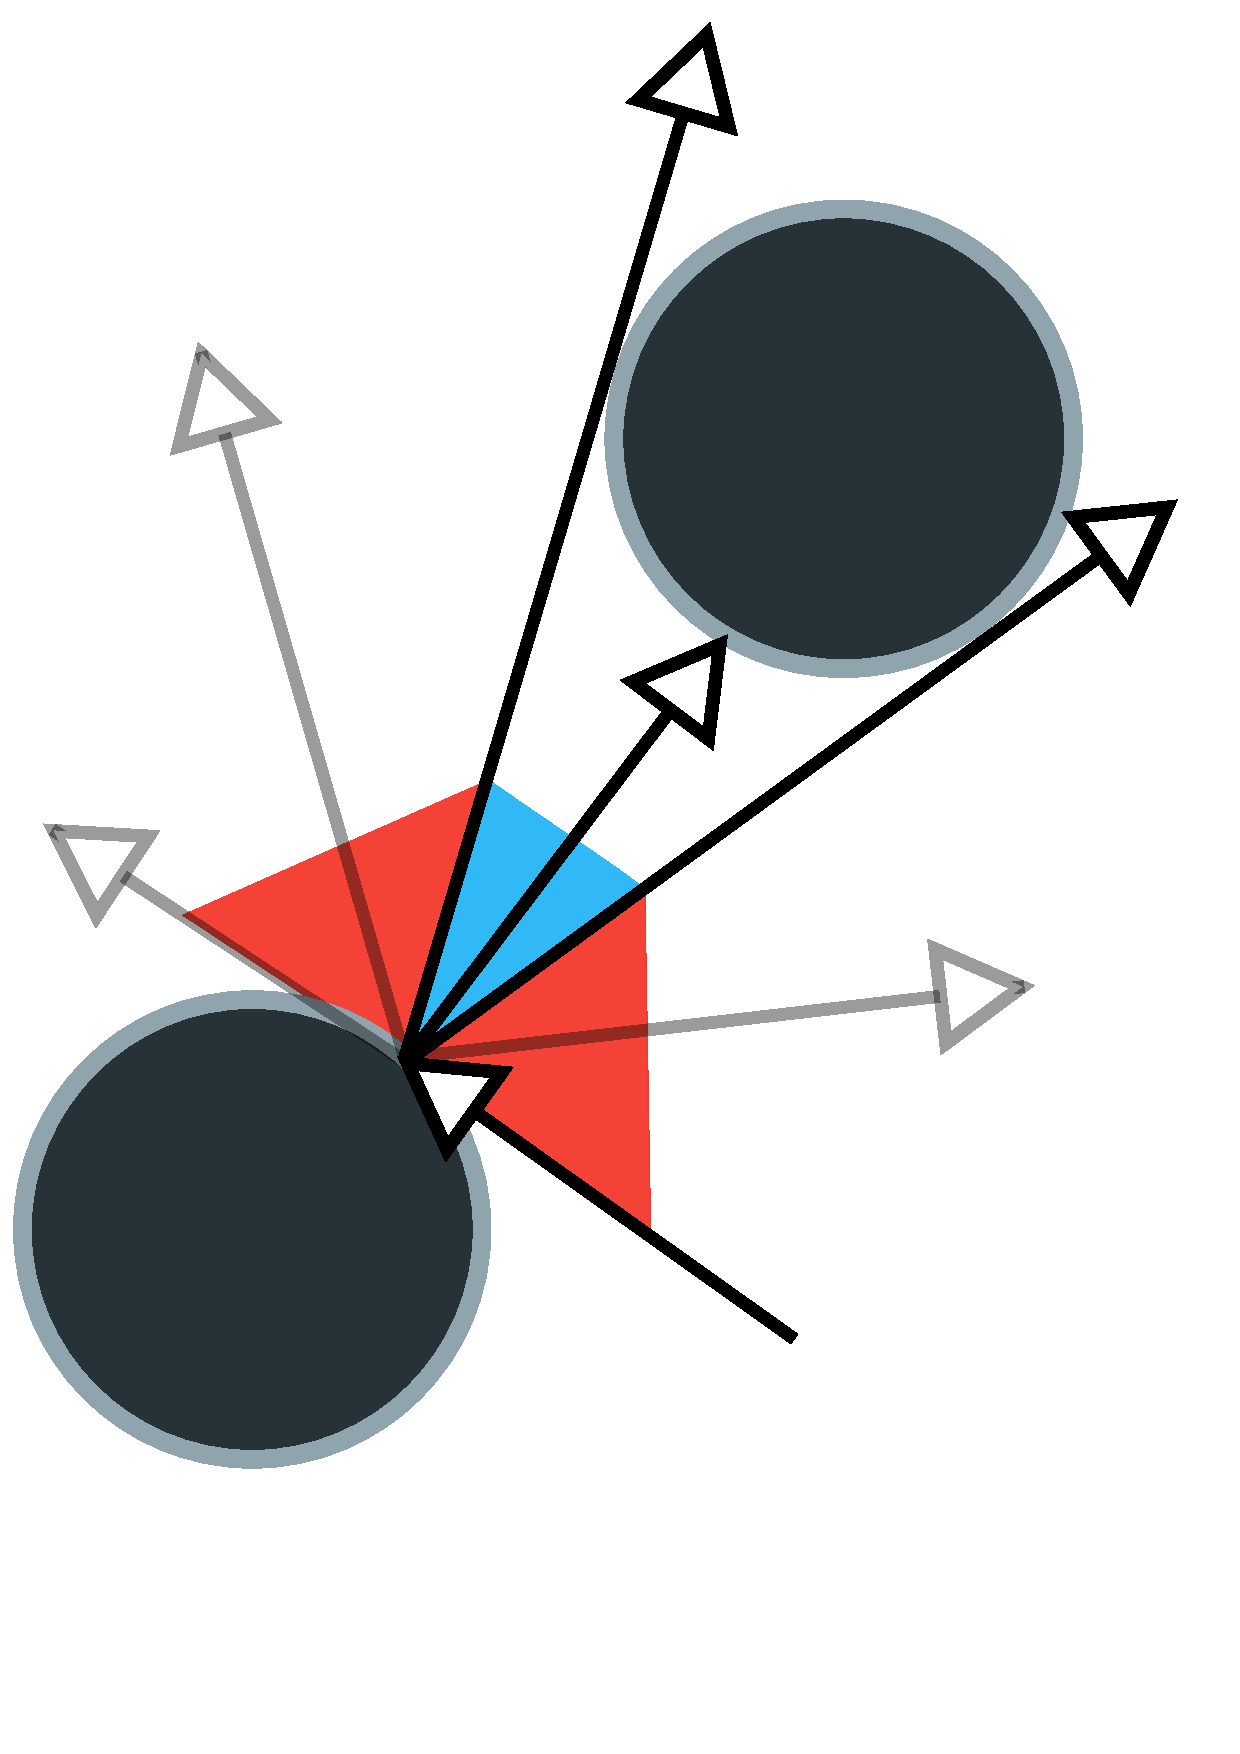
\includegraphics[height=180px]{res/raytrace.pdf}
\column{0.6\linewidth}
{\scriptsize
\begin{code}
  -- | recursively raytrace
  raytrace :: Ray -> Rand Color
  raytrace r = do
    case getCollision r of
      Some (surface, loc) -> 
       color' <- averageRays loc
       return $ mixColor surface color'
      None -> return backgroundColor

  -- | Send a random ray 
  sendRandRay :: Position -> Rand Color
  sendRandRay p =
    u <- uniform01
    let angle = 360 * u
    raytrace (makeRay p angle)

  -- | Average rays sent from a location
  averageRays :: Position -> Rand Color
  averageRays p = do
    -- | computationally wasteful
    colors <- replicateM 100 (sendRandRay p)
    return $ averageColors colors

  -- | Default background color.
  backgroundColor = white
\end{code}
}
\end{columns}
\end{frame}

\begin{frame}[fragile]{Raytracing (Scored)}
\begin{columns}
\column{0.5\linewidth}
{\scriptsize
\begin{code}
  raytrace :: Ray -> Rand Color
  raytrace r = do
    case getCollision r of
      Some (surface, loc) -> 
       color' <- averageRays loc
       return $ mixColor surface color'
      None -> return backgroundColor
\end{code}
}

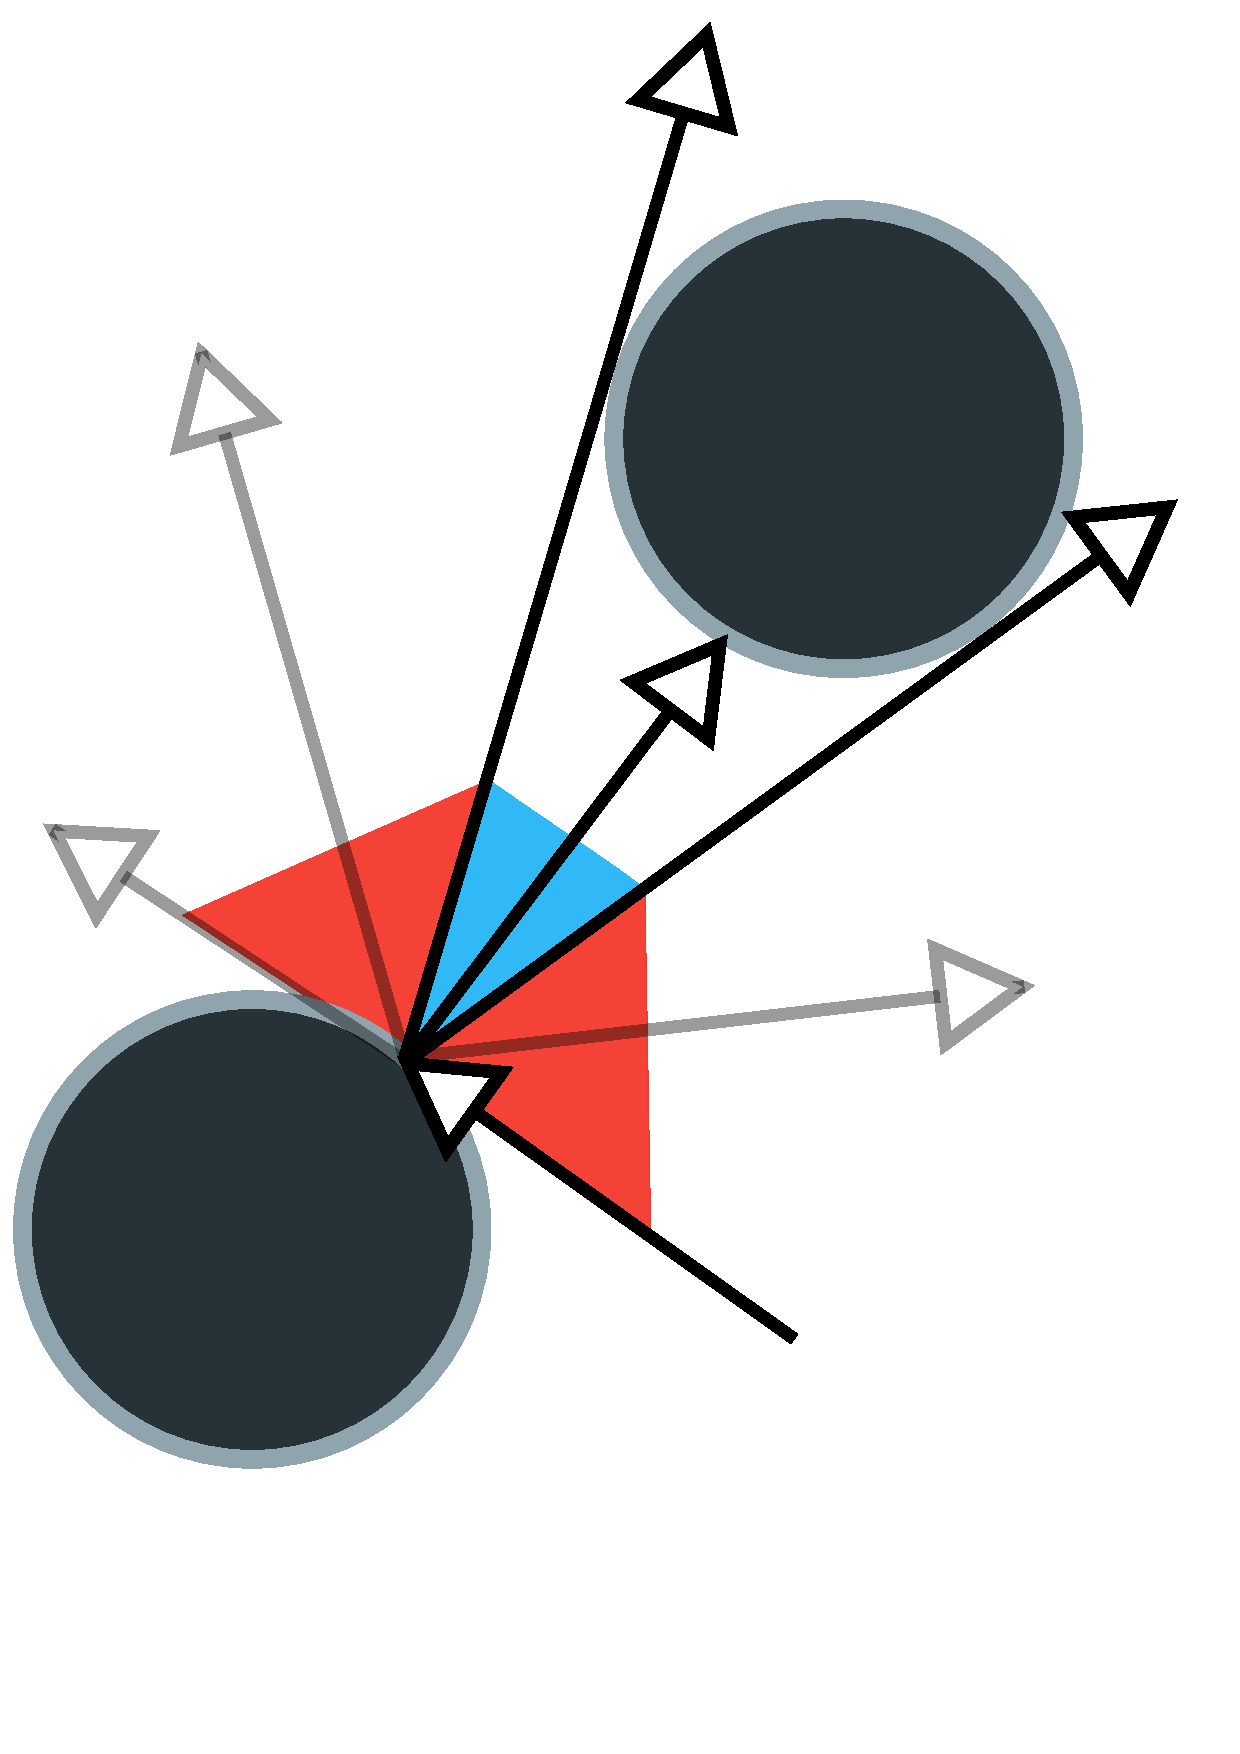
\includegraphics[height=180px]{res/raytrace.pdf}
\column{0.5\linewidth}
{\scriptsize
\begin{code}
  raytrace' :: Ray -> Rand Color
  raytrace' r = do
    case getCollision r of
      Some (surface, loc) -> 
       color' <- averageRays loc
       return $ mixColor surface color'
      None -> do
        score 0.5 -- New! 
        return backgroundColor
\end{code}
}
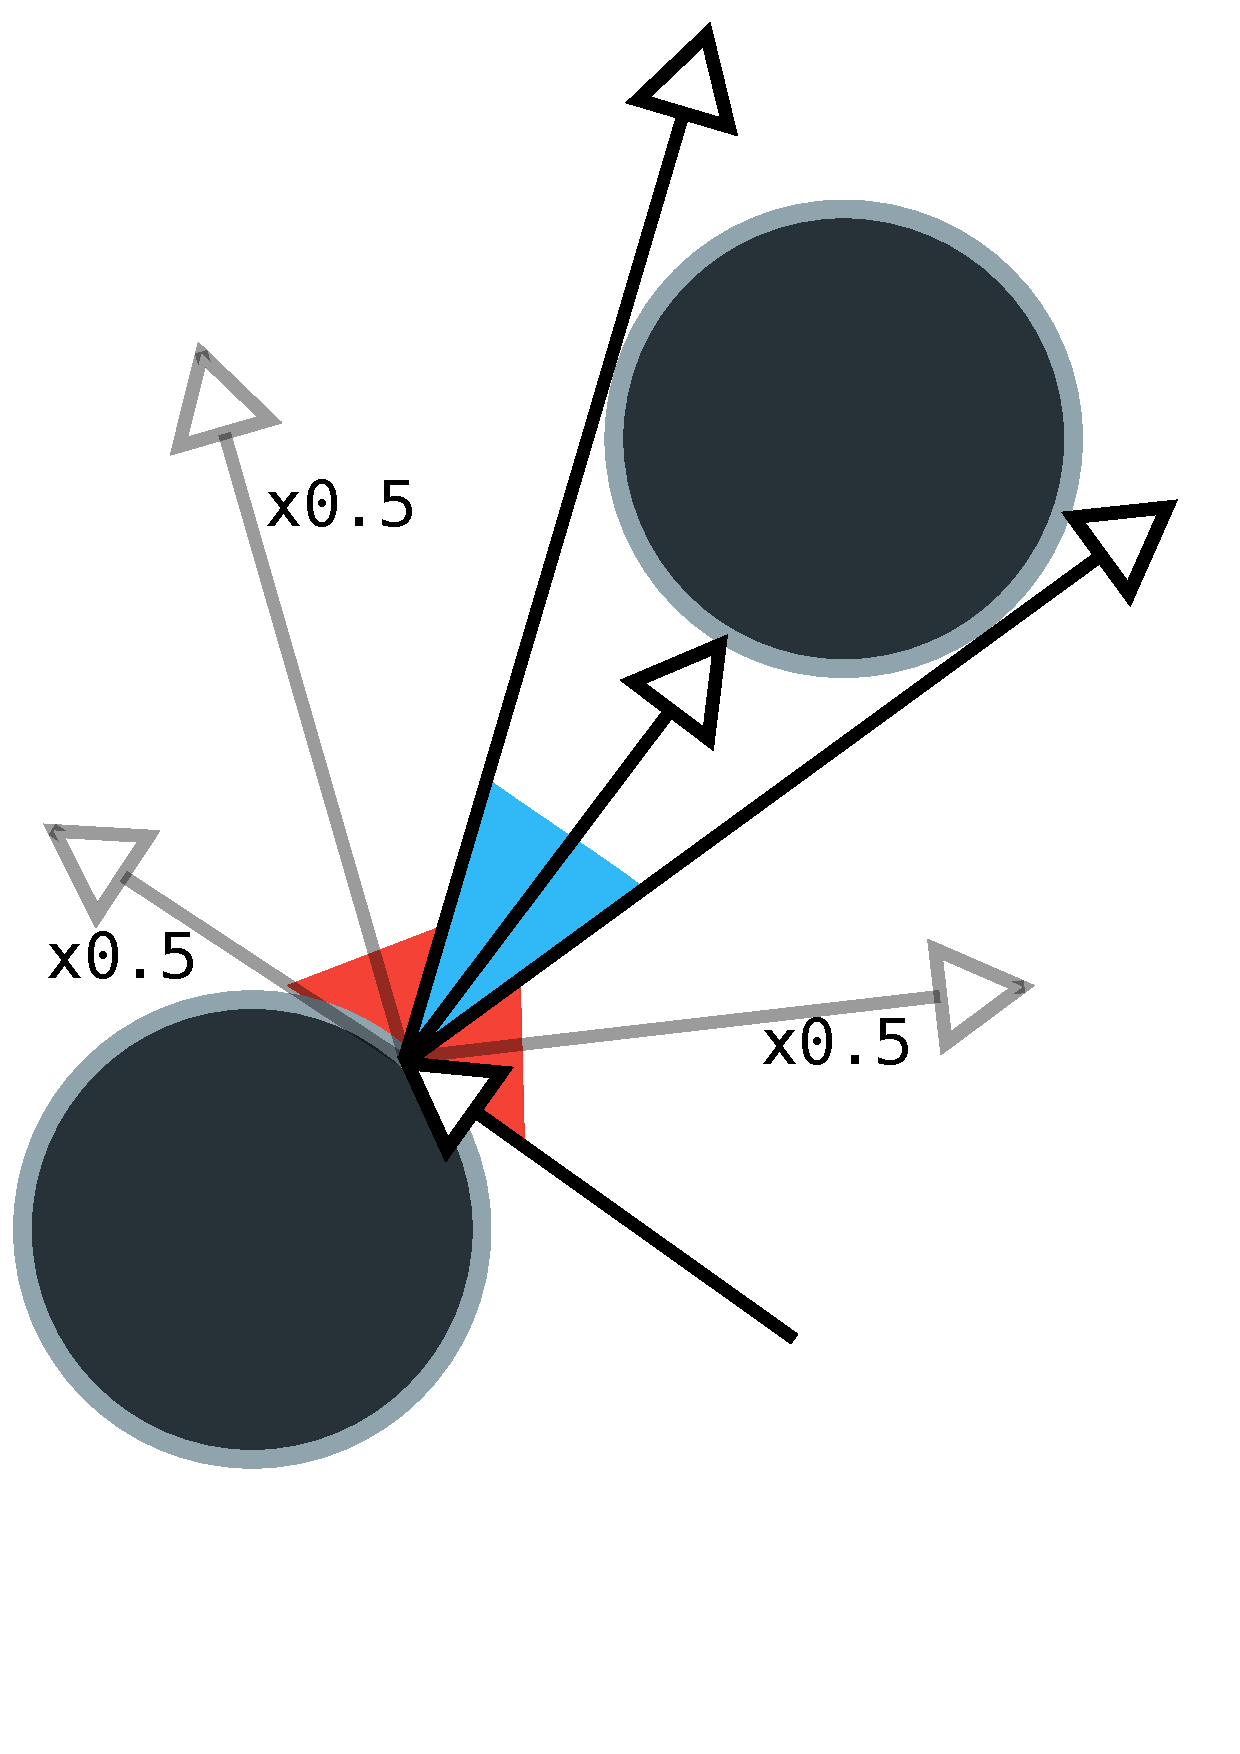
\includegraphics[height=180px]{res/raytrace-scored.pdf}
\end{columns}
\end{frame}

\begin{frame}[fragile]{Program optimisation (Uniform)}
\begin{columns}
\column{\linewidth}
{\scriptsize \footnotesize
\begin{code}
-- | Randomly change programs and return their performance
equivRandomProgram :: Program -> Rand (Performance, Program)
equivRandomProgram p = do
  p' <- modifyProgram p
  if semanticsEqual p p'
  then return (performance p', p')
  else return (0, p') -- A program that does not work has 0 perf.

-- | Take the random samples and pick the good performing ones
optimise :: Program -> Program
optimise p = 
  let ps' = sample 100 (equivRandomProgram p)
  in snd $ maximumBy (compare . fst) ps'
\end{code}
}
\end{columns}
\end{frame}


\begin{frame}[fragile]{Program optimisation (Scored)}
\begin{columns}
\column{\linewidth}
{\scriptsize \footnotesize
\begin{code}
equivRandomProgram' :: Program -> Rand (Performance, Program)
equivRandomProgram' p = do
 (perf, p) <- equivRandomProgram p
 let perf = 
    if semanticsEqual p p'
      then performance p'
      else 0
 score perf -- ^ Correct programs are more likely
 return (perf, p')

equivRandomProgram :: Program -> Rand (Performance, Program)
equivRandomProgram p = do
  p' <- modifyProgram p
  if semanticsEqual p p'
  then return (performance p', p')
  else return (0, p') -- A program that does not work has 0 perf.
\end{code}
}

{\scriptsize \tiny
    \texttt{http://stoke.stanford.edu/}\qquad
    \texttt{https://github.com/bollu/blaze/blob/master/notebooks/tutorial.ipynb}
}
\end{columns}
\end{frame}



\begin{frame}[fragile]{Learning from prior experience}

\begin{code}
-- | Naive understanding, in the beginning of the process
prior :: Rand a
prior = ...

-- | Learn as you go!
learn :: Rand a
learn = do
  value <- prior
  score (usefulness value)
  return value
\end{code}

\end{frame}

\begin{frame}[fragile]{Motivation}

\begin{code}
-- | fair dice
dice :: Rand Int
dice = choose [1, 2, 3, 4, 5, 6]

tossDice :: Rand Int
tossDice = do
    d1 <- dice
    d2 <- dice
    return $ d1 + d2
\end{code}

\input{"| cabal v2-exec slides -- tossDice"}

If the dice roll is prime, 

\begin{code}
tossDicePrime :: Rand Int
tossDicePrime = do
    d <- tossDice
    score $ if prime d then 1 else 0
    return $ d
\end{code}

\input{"| cabal v2-exec slides -- tossDicePrime"}
  
\end{frame}

\begin{frame}[fragile]
\begin{code}
data Rand x where
    Ret :: x -> Rand x
    SampleUniform01 :: (Double -> Rand x) -> Rand x
    Score :: Double -> Rand x -> Rand x
\end{code}
\end{frame}

\begin{comment}
\begin{code}
instance Functor Rand where
  fmap f (Ret x) = Ret (f x)
  fmap f (SampleUniform01 r2mx) = SampleUniform01 (\r -> fmap f (r2mx r))
  fmap f (Score s mx) = Score s (fmap f mx)
instance Applicative Rand where
  pure = Ret
  (<*>) = ap 
instance Monad Rand where
  return = Ret
  (Ret x) >>= x2my = x2my x
  (SampleUniform01 r2mx) >>= x2my = SampleUniform01 (\r -> r2mx r >>= x2my)
  (Score s mx) >>= x2my = Score s (mx >>= x2my)
\end{code}
\end{comment}

\begin{frame}[fragile]
\begin{code}
-- | Run the computation _unweighted_.
-- | Ignores scores.
sample :: RandomGen g => g -> Rand a -> (a, g)
sample g (Ret a) = (a, g)
sample g (SampleUniform01 f2my) =
  let (f, g') = random g in sample g' (f2my f)
sample g (Score f mx) = sample g mx -- Ignore score
\end{code}
\end{frame}

\begin{frame}[fragile]
MCMC methods
\end{frame}

\begin{frame}[fragile]
\begin{code}
-- | Trace all random choices made when generating this value
data Trace a =
  Trace { tval :: a, -- ^ The value itself
          tscore :: Double, -- ^ The total score
          trs :: [Double] -- ^ The ranom numbers used
        }
-- | Lift a pure value into a Trace value
mkTrace :: a -> Trace a
mkTrace a = Trace a 1.0 []
-- | multiply a score to a trace
scoreTrace :: Double -> Trace a -> Trace a
scoreTrace f Trace{..} = Trace{tscore = tscore * f, ..}
-- | Prepend randomness
recordRandomness :: Double -> Trace a -> Trace a
recordRandomness r Trace{..} = Trace { trs = r:trs, ..}

-- | Trace a random computation.
-- We know what randomness is used
traceR :: Rand x -> Rand (Trace x)
traceR (Ret x) = Ret (mkTrace x)
traceR (SampleUniform01 mx) = do
  r <- sample01
  trx <- traceR $ mx r
  return $ recordRandomness r $ trx
traceR (Score s mx) = do
  trx <- traceR $ mx
  return $ scoreTrace s $ trx
\end{code}
\end{frame}


-- | Return a trace-adjusted MH computation
\begin{frame}[fragile]
\begin{code}

  
mhStep :: Rand (Trace x) -- ^ proposal
         -> Trace x -- ^ current position
         -> Rand (Trace x)
mhStep r trace = do
  -- | Return the original randomness, perturbed
  rands' <- perturbRandomness (trs trace)
  -- | Run the original computation with the perturbation
  trace' <- feedRandomness rands' r
  let ratio = traceAcceptance trace' / traceAcceptance trace
  r <- sample01
  return $ if r < ratio then trace' else trace
  
traceAcceptance :: Trace x -> Double
traceAcceptance tx =
  tscore tx * fromIntegral (length (trs tx))
  
perturbRandomness :: [Double] -> Rand [Double]
perturbRandomness rands = do
  ix <- choose [0..(length rands-1)] -- ^ Random index
  r <- sample01 -- ^ random val
  -- | Replace random index w/ random val.
  return $ replaceListAt ix r rands 
\end{code}
\end{frame}

\begin{frame}[fragile]
\begin{code}
-- | Find a starting position that does not have probability 0
findNonZeroTrace :: Rand (Trace x) -> Rand (Trace x)
findNonZeroTrace tracedR = do
  trace <- tracedR
  if tscore trace /= 0
  then return $ trace
  else findNonZeroTrace tracedR

-- | run the computatation after taking weights into account
weighted :: MCMC x => Int -> Rand x -> Rand [x]
weighted 0 _ = return []
weighted n r =
  let tracedR = traceR r
      -- go :: Int -> Rand (Trace x) -> Rand (Trace [x])
      go 0 _ = return []
      go n tx = do
        tx' <- repeatM 10 (mhStep tracedR) $ tx
        txs <- go (n-1) tx'
        return (tx:txs)
  in do
      seed <- findNonZeroTrace $ tracedR
      tracedRs <- go n seed 
      return $ map tval tracedRs
\end{code}
\end{frame}

\begin{frame}[fragile]{Payoff!}
\begin{code}
predictCoinBias :: [Int] -> Rand Double
predictCoinBias flips = do
  b <- sample01
  forM_ flips $ \f -> do
    -- | Maximum a posterior
    score $ if f == 1 then b else (1 - b)
  return $ b
\end{code}

\begin{code}
predictCoinBiasNoData :: Rand Double
predictCoinBiasNoData = predictCoinBias []
\end{code}

\input{"| cabal v2-exec slides -- predictCoinBiasNoData"}


\begin{code}
predictCoinBias0 :: Rand Double
predictCoinBias0 = predictCoinBias [0]
\end{code}

\input{"| cabal v2-exec slides -- predictCoinBias0"}

\begin{code}
predictCoinBias01 :: Rand Double
predictCoinBias01 = predictCoinBias [0, 1]
\end{code}

\input{"| cabal v2-exec slides -- predictCoinBias01"}

\end{frame}


\begin{frame}[fragile]{More fun stuff: sample from arbitrary distributions}

\begin{code}
sampleSinSq :: Rand Double
sampleSinSq = do
  x <- (6 *) <$> sample01
  score $ (sin x) * (sin x)
  return $ x
\end{code}

\input{"| cabal v2-exec slides -- sampleSinSq"}

\end{frame}


\begin{frame}[fragile]{Transformations discovered by \texttt{STOKE}}
\begin{columns}
\column{\linewidth}
{\scriptsize
\begin{ascii}
// constant folding: 2 + 3 -> 5
*** original: (nparams: 0 | [IPush 2,IPush 3,IAdd])***
[IPush 5] | score: 2.5

// strength reduction: 2 * x -> x + x
*** original: (nparams: 1 | [IPush 2,IMul])***
[IDup,IAdd] | score: 2.25 

// algebraic rewrite: x & x == x
*** original: (nparams: 1 | progInsts = [IDup,IAnd])***
[] | score: 3.0
\end{ascii}
}
\end{columns}

\end{frame}
\end{document}


